%-----------------------------------------------------------
%              TABLA DE NOMENCLATURA
%------------------------------------------------------
\graphicspath{ {W_Varios/0_Tablas_notacion/img/ejemplos/}, {img/} }
\begin{center}
	\section*{i. Tabla de nomenclatura }
	\addcontentsline{toc}{section}{i. Tabla de nomenclaturas }
\end{center}

\begin{spacing}{1}
	\begin{center}
		\begin{tabular}{ |p{2.5cm}|p{9.5cm}|}
			\hline
			\rowcolor{orange!50}
			\begin{center} \textbf{Siglas} \end{center} & \begin{center}

				\textbf{Nombre}\end{center}                                                           \\ \hline
			
			EA                        & Efectivo Anual (tasa de referencia SuperFinanciera-nominal anual año vencido- naav) \\ \hline
			
			g                         & Gradiente geométrico                                                                \\ \hline
			
			H                         & Valor incremento escalón monetario                                                  \\ \hline
			
			I                         & Monto de interés                                                                    \\ \hline
			
			IPC                       & Índice de precios al consumidor                                                     \\ \hline
			
			L                         & Gradiente aritmético monetario                                                      \\ \hline
			
			$i$                       & Tasa de interés periódico                                                           \\ \hline
			
			$j$                       & Tasa de interés periódica anualizada                                                \\  \hline
			
			i$_{d}$                   & Tasa periódica de devaluación                                                       \\ \hline
			i$_{f}$                   & Tasa periódica de la inflación                                                      \\ \hline
			i$_{r}$                   & Tasa periódica real                                                                 \\ \hline
			
			m$_{1}$                   & Número de períodos anuales para  i$_{1}$                                            \\ \hline
			
			m$_{2}$                   & Número de períodos anuales para  i$_{2}$                                            \\ \hline
			
			n                         & Número de periodos asociados a una i                                                \\ \hline
			
			na(120d)v                 & Nominal anual (120 días) vencido                                                    \\ \hline
			
			naaa                      & Nominal anual (año) anticipado                                                      \\ \hline
			
			naav                      & Nominal anual (año) vencido                                                         \\ \hline
			
			nasa                      & Nominal anual (semestre) anticipado                                                 \\\hline
			
			nasv                      & Nominal anual (semestre) vencido                                                    \\\hline
			
			nata                      & Nominal anual (trimestre) anticipado                                                \\ \hline
			
			natv                      & Nominal anual (trimestre) vencido                                                   \\ \hline
			
			na(5a)a                   & Nominal anual (5 años) anticipado                                                   \\ \hline
			
			na(5a)v                   & Nominal anual (5 años) vencido                                                      \\ \hline
			
			na(120d)a                 & Nominal anual (120 días) anticipado                                                 \\ \hline
			
			p(120d)v                  & Periódico (120 días) vencido                                                        \\ \hline
			
			paa                       & Periódico (año)  anticipado                                                         \\ \hline
			
			pav                       & Periódico (año) vencido                                                             \\ \hline
			
			psa                       & Periódico (semestre) anticipado                                                     \\\hline
			
			psv                       & Periódico (semestre) vencido                                                        \\\hline
			
			pta                       & Periódico (trimestre) anticipado                                                    \\ \hline
			
			ptv                       & Periódico (trimestre) vencido                                                       \\ \hline
			
			p(5a)a                    & Periódico (5 años) anticipado                                                       \\ \hline
			
			p(5a)v                    & Periódico (5 años) vencido                                                          \\ \hline
			
			p(120d)a                  & Periódico (120 días) anticipado                                                     \\ \hline
			
			R                         & Cuotas seriales fijas                                                               \\ \hline
			
			SPREAD                    & Tasa de interés que se adiciona a una tasa de referencia                            \\ \hline
		\end{tabular}
	\end{center}
\end{spacing}
\ \ \
%\begin{center}
%\section*{Aceptaciones Bancarias}
%\addcontentsline{toc}{section}{Tabla resumen de fórmulas }
%\end{center}
\\ \\ \\ \\ \\ \\ \\
\begin{center} \textbf {Aceptaciones Bancarias (capítulo 3)}\\ \end{center}

\begin{spacing}{1}
	\begin{center}
		\begin{tabular}{ |p{2.5cm}|p{9.5cm}|}
			\hline
			\rowcolor{orange!50}
			\begin{center}\textbf{Siglas} \end{center} & \begin{center} \textbf{Nombre} \end{center}                                                                                                                                                                                                           \\ \hline
			
			
			COM$_{v}$                 & Comisión de Venta del Corredor                                                                                                                                                                                                      \\ \hline
			i$_{c}$                   & Tasa de compra                                                                                                                                                                                                                      \\ \hline
			i$_{R}$                   & Tasa de registro en Bolsa de Valores                                                                                                                                                                                                \\ \hline
			i$_{v}$                   & Tasa de venta                                                                                                                                                                                                                       \\ \hline
			P$_{c}$                   & Precio del comprador                                                                                                                                                                                                                \\ \hline
			P$_{R}$                   & Precio de registro                                                                                                                                                                                                                  \\ \hline
			P$_{v}$                   & Precio de venta                                                                                                                                                                                                                     \\ \hline
			$*$                       & Para las ecuaciones de valor el * es un operador que multiplica o desplaza un flujo y/o el resultado del flujo de series uniformes y/o gradiantes diferidos y/o con tiempo muerto (único caso de uso de este operador en esta guía. \\ \hline
		\end{tabular}
	\end{center}
\end{spacing}



\begin{center} \textbf {Operadores lógicos} \end{center}

\begin{spacing}{1}
	\begin{center}
		\begin{tabular}{ |p{2.5cm}|p{9.5cm}|}
			\hline
			\rowcolor{orange!50}
			\begin{center}\textbf{Siglas} \end{center} & \begin{center} \textbf{Nombre} \end{center}                                 \\ \hline
			
			$ Q \Leftarrow P $        & "Q dado que P", "Q si P", "Q siempre que P"               \\ \hline
			
			$ P \Rightarrow Q $       & "P implica Q", "Si P, entonces Q", "P sólo si Q"          \\ \hline
			
			$ P \Leftrightarrow Q $   & "P si y sólo si Q", "P es necesario y suficiente para Q", 
			"P es equivalente con Q"                                                              \\ \hline
			
			$ \therefore P $         & "Porque P"                                                \\ \hline
			
			$ \therefore  P $         & "Por lo tanto, P"                                         \\ \hline
			
			$\equiv$                  & Equivalente                                               \\ \hline
		\end{tabular}
	\end{center}
\end{spacing}
\newpage
%-----------------------------------------------------------
%              TABLA DE FORMULAS
%------------------------------------------------------

\begin{center}
	\section*{ii. Tabla resumen de fórmulas}
	\addcontentsline{toc}{section}{ii. Tabla resumen de fórmulas trabajadas en la guía}
\end{center}

\begin{spacing}{1}
	\begin{center}
		\begin{tabular}{ |p{7cm}|p{7cm}|}
			\hline
			\rowcolor{orange!50}
			
			\begin{center}\textbf{Fórmula} \end{center}                                                                   & \begin{center} \textbf{Nombre} \end{center}                                 \\ \hline
			
			$(1 + i_{1})^{m_1} = (1 + i_{2})^{m_2}$                                                      & Equivalencia de tasas periódicas                           \\\hline
			
			$i_{r} = i_{1} + i_{2} + i_{1}i_{2}$                                                         & Tasa de interés periódica real                             \\ \hline
			$i_r = \frac{i - i_f}{1 + i_f}$                                                              & Tasa de interés real                                       \\ \hline
			
			$j = im$                                                                                     & Tasa interés nominal anual vencida                         \\ \hline
			
			
			$i_a = \frac{i}{1 + i}$                                                                      & Tasa de interés periódica anticipada                       \\ \hline
			
			$i = \frac{i_a}{1 - i_a}$                                                                    & Tasa de interés periódica vencida                          \\ \hline
			$D = Fdn$                                                                                    & Valor de descuento dado un flujo (F)                       \\ \hline
			
			$F = P(1 + i)^n$                                                                             & Valor futuro                                               \\ \hline
			
			$VP = R  \frac{1-(1 + i)^{-n}}{i} $                                                          & Valor presente serie uniforme vencida                      \\ \hline
			
			$VP_{a} = R  \frac{1-(1 + i)^{-n}}{i}  (1 + i) $                                             & Valor presente serie uniforme anticipada                   \\ \hline
			
			$VF = R  \frac{(1 + i)^n-1}{i} $                                                             & Valor futuro serie uniforme vencida                        \\ \hline
			$VF_{a} = R  \frac{(1 + i)^n-1}{i}(1 + i) $                                                  & Valor futuro serie uniforme anticipada                     \\ \hline
			
			$VP = \frac{R}{i}$                                                                           & Valor presente serie perpetua vencida                      \\ \hline
			$VP = R  \frac{1-(1 + i)^{-n}}{i} + \frac{L}{i}[ \frac{1-(1 + i)^{-n}}{i} - n(1 + i)^{-n} ]$ & Valor presente de gradiente aritmético                     \\ \hline
			$VF = R  \frac{(1 + i)^{n} - 1}{i} + \frac{L}{i}[ \frac{(1 + i)^n - 1}{i} - n ]$             & Valor futuro de gradiente aritmético                       \\ \hline
			$VP = \frac{R}{i} + \frac{L}{i^2}$                                                           & Valor presente gradiente aritmético infinito               \\ \hline
			$VP = R  \frac{(1 + g)^n  (1 + i)^{-n}-1}{g - i} $                                           & Valor presente de gradiente geométrico, si $g \neq i$      \\ \hline
			$VP = \frac{Rn}{1 + i}$                                                                      & Valor presente gradiente geométrico si $g = i$             \\ \hline
			$VF = R  \frac{(1 + g)^n - (1 + i)^n}{g - i} $                                               & Valor futuro gradiente geométrico si $g \neq i$            \\ \hline
			$VF = Rn(1 + i)^{n-1} $                                                                      & Valor futuro gradiente geométrico si $g = i$               \\ \hline
			$VP = \frac{R}{1 - g} $                                                                      & Valor presente gradiente geométrico infinito si $g < i$    \\ \hline
			$VP = \infty $                                                                               & Valor presente gradiente geométrico infinito si $g \geq i$ \\ \hline
		\end{tabular}
		
		\clearpage
		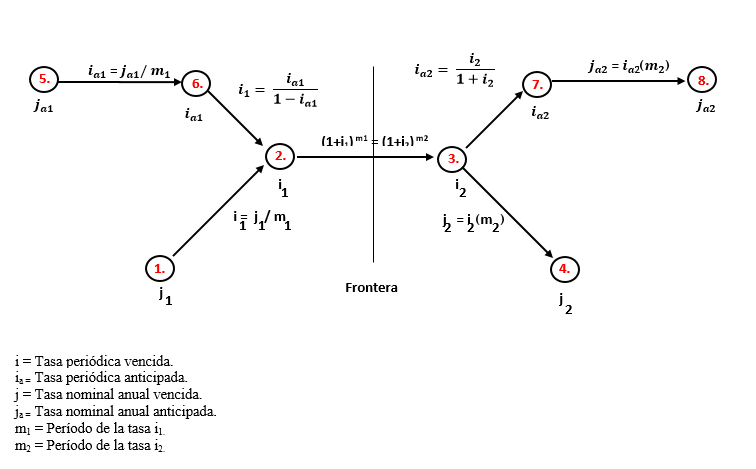
\includegraphics[width = 10.0 cm]{general}\\
		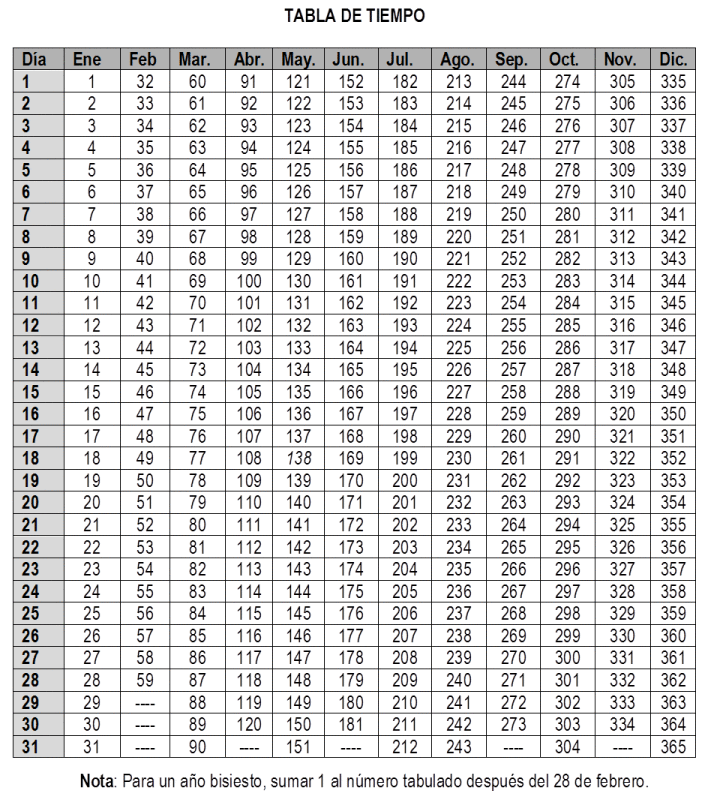
\includegraphics[height=15cm]{TTime}
	\end{center}
\end{spacing}

\clearpage

\begin{center}
	\section*{iii. Tabla resumen de fórmulas}
	\addcontentsline{toc}{section}{iii. Tabla funciones de Excel}
\end{center}

\vspace{2cm}

\begin{spacing}{1}
	\begin{center}
		\begin{tabular}{ |p{7cm}|p{5.5cm}|}
			\hline
			\rowcolor{orange!50}
			
			\begin{center}\textbf{Nombre} \end{center}             & \begin{center} \textbf{Función Financiera en Excel} \end{center} \\ \hline
			
			Equivalencia de tasas periódicas       & TASA(m;;-1;1+i)            \\\hline
			
			Tasa interés nominal anual vencida     & TASA.NOMINAL(i;m)          \\ \hline
			
			Tasa interés periódica año vencido     & INT.EFECTIVO(j;m)          \\ \hline
			
			Valor futuro                           & VF(i;n;;VA,0)              \\ \hline
			
			Valor presente                         & VA(i;n;;VF,0)              \\ \hline
			
			Valor presente serie uniforme vencida  & VNA(i;R1;R2;R3;...)        \\ \hline
			
			Valor futuro serie uniforme vencida    & VF(i;n;;VA,0)              \\ \hline
			
			Valor futuro serie uniforme anticipada & VF(i;n;;VA,1)              \\ \hline
			
			Valor presente serie perpetua vencida  & VA(i;n;R;0)                \\ \hline
			
			Valor presente gradiente aritmético    & VNA(i;R1;R2;R3;...)        \\ \hline
			
			Valor presente gradiente geométrico    & VNA(i;R1;R2;R3;...)        \\ \hline
			
			Valor cuota serie uniforme vencida     & PAGO(i;n;P;F;0)            \\ \hline
			
			Valor cuota serie uniforme anticipada  & PAGO(i;n;P;F;1)            \\ \hline
			
			Ecuación de valor                      & Función Buscar Objetivo    \\ \hline
		\end{tabular}
	\end{center}
\end{spacing}

\clearpage
